\chapter{Evaluation}

\label{Chapter6}

In order to evaluate the performance of the forked version of Moonlight developed for this paper, it must be tested against the other existing solutions.
The testing methodology employed to ensure the accuracy of the testing is described in Section \ref{sec:TestingMethodology}.
Then, the different results are evaluated and analyzed in Sections \ref{sec:ResponsivityAndLatency} and \ref{sec:Quality}.
Finally, the results are summarized and verdicts on each of the solutions' applicability to the research questions will be presented in Section \ref{sec:EvaluationSummary}.


\section{Testing Methodology}\label{sec:TestingMethodology}

In order to ensure that the data collected for analysis is accurate and directly comparable, the testing environment must be kept exactly the same between trials and between different applications.
This gives each application the exact same starting conditions, and the best chance to demonstrate it's unabated performance.
For these tests, the host machine is a desktop computer running Windows 10 with a AMD Ryzen 9 5900X CPU and a Nvidia RTX 3070 GPU running the latest GeForce Experience version \emph{3.25.0.84}.
This configuration does not change throughout testing.
The client machine is the CM4 board attached to the PCB developed in Chapter \ref{Chapter4}, running the custom Manjaro linux distribution and forked version of Moonlight developed in Chapter \ref{Chapter5}.
This configuration also does not change throughout testing.
Each test is performed with both the host computer and the client machine running on the same network, with both devices connected to the same router using an ethernet cable.
This ensures that the speed of the network is not a factor in the tests.
The tests are performed multiple times under the following conditions:

\begin{itemize}
  \item Ideal Conditions: No other applications are running during testing.
  \item CPU Stressed: The CPU is constantly at 100\% load during the entire test.
  \item GPU Stressed: The GPU is constantly at 100\% load during the entire test.
\end{itemize}

\noindent
This is to examine whether each application can perform under intensive conditions.
For each test, the following steps are performed:

\begin{enumerate}
  \item Both the host and client computers are fully rebooted to ensure no other application is running.
  \item The host computer starts up a single browser window with the web page described in Section \ref{sec:DevelopingTestingAndMeasurementTools}.
  \item If the test calls for the CPU or the GPU to be stressed, the application \enquote{Blender} is started on the host machine, and a benchmark is performed for the CPU or the GPU.
        This benchmark will run for longer than the duration of the test, and will keep the CPU or GPU at 100\% load for the entire duration of the benchmark.
  \item Both devices start up their respective data collection tool that will record key-strokes and changes in the screen's color.
  \item The client machine connects to the host computer using the application being tested.
  \item The tester presses the \enquote{0} key on the client's numpad to synchronize the two devices' clocks and data recording tools (Detailed below).
  \item The tester begins by typing on the client's keyboard at a steady pace as close to 50 words per minute as possible, allowing both computers to record their data.
  \item The tester then types on the client's keyboard at a quicker pace of approximately 100 words per minute to ensure that quick successive inputs are handled correctly and no data is lost or duplicated.
  Due to the wide variance in what the user can do using the software, it is nearly impossible to test real world scenarios.
  Instead, high frequency inputs coupled with updating the entire screen mimic high-intensity applications.
  \item Once typing is complete, both the client and the host computers close their data recording tools and the client ends the streaming session.
\end{enumerate}

\noindent
This process is repeated for each of the following applications:

\begin{itemize}
  \item The forked version of Moonlight developed for this project.
  \item Chrome Remote Desktop (CRD, Section \ref{subsec:ChromeRemoteDesktop}).
  \item Microsoft's Remote Desktop Connection (RDP, Section \ref{subsec:RemoteDesktopProtocol}).
  \item Virtual Network Computing (VNC, Section \ref{subsec:VirtualNetworkComputing}).
\end{itemize}

\noindent
Once all the data is collected, the data from the host and client machines for a single trial are organized into a single CSV file for processing.
In order to ensure that the data is comparable, all extraneous factors must be removed from the data.
Namely, the network latency and difference in computer clocks must be removed.
By keeping the host and client computers attached to the same network through ethernet, the network latency is minimized.
But the task of keeping two computer's internal clocks synchronized is not trivial.
Even after instructing the operating system to synchronize its clock with an internet time server, the two computers may still report different times.
In some cases, the difference between the host and client computer's system time was noticed to be upwards of a full second after resynchronizing both clocks \cite{time.is}.
This is partially accounted for in step \emph{6} of the above process, and the remaining inaccuracy can now be removed by subtracting the time difference between the when the client presses the button and the time the host executes that command.
This ensures that any inaccuracies in each computer's internal clock will not impact the data.

After the data is cleaned up, the data can be processed by matching each key-stroke and change in the screen's color detected by the client and host machines and calculating how much time elapsed between the events.
This reveals the amount of delay the user experiences between when they press a key and when the host executes the command, and between when they press a key and can visually see the response.


\section{Responsivity and Latency}\label{sec:ResponsivityAndLatency}

The first factor in determining the performance of the application is to take a look at how responsive it is to use.
Responsivity is defined as how quick the application responds to inputs and how quickly the user can see the results of their inputs.
This is important for general user experience and applications where continuous input is required.
This is also what is generally referred to when determining whether an application has a positive user experience, since a program that can take seconds to respond to the user begets lower productivity and a more frustrating experience.
To analyze this, two points of data are recorded: First, the amount of time between when the client records a keystroke and when it is actually inputted on the host machine, and secondly, the amount of time between the host machine updating their screen and when the client actually displays that update.
The first datum is generally referred to as the latency of the application, since even though each trial is done using the same network setup different programs may have different optimizations built in that reduce the time needed for the host to implement keystrokes made by the client.
Each of the following figures shows data over one trial for each category.
Each trial lasted approximately 60 seconds following the steps detailed in Section \ref{sec:TestingMethodology}, totaling to approximately 200 keystrokes per trial.
Limitations in this data is discussed in Section \ref{sec:ConclusionLimitations}.
Figure \ref{fig:InputDelay} shows the amount of time between the client and the host registering the keystroke under the different test conditions.

\begin{figure}[h]
  \centering
  \begin{tikzpicture}
    \begin{axis}[
      boxplot/draw direction=y,
      ylabel={Time (ms)},
      scale only axis,
      height=8cm,
      width=\textwidth,
      ymin=0,ymax=200,
      cycle list={{black},{blue},{red}},
      legend style={
          legend pos=outer north east,
          font=\small
        },
      legend cell align=left,
      legend image code/.code={%
          \draw[#1] (0cm,-0.1cm) rectangle (0.6cm,0.1cm);
        },
      boxplot={
          % Three boxplots for each column
          draw position={1/4 + floor(\plotnumofactualtype/3) + 1/4*mod(\plotnumofactualtype,3)},
          % Each plot takes up a quarter of the column
          box extend=0.2,
        },
      % 1 unit in x controls the width:
      x=2cm,
      % ... and it means that we should describe intervals:
      xtick={0,1,2,...,10},
      x tick label as interval,
      xticklabels={%
      {Forked Moonlight\\{\tiny ideal/cpu/gpu}},%
      {CRD\\{\tiny ideal/cpu/gpu}},%
      {RDP\\{\tiny ideal/cpu/gpu}},%
      {VNC\\{\tiny ideal/cpu/gpu}},%
      },
      x tick label style={
          text width=2.5cm,
          align=center
        },
      ]

      % Forked Moonlight
      \addplot
      table[col sep=comma,x=Time difference] {Data/ideal/moonlight_key_delay.csv};
      \addplot
      table[col sep=comma,x=Time difference] {Data/stresscpu/moonlight_key_delay.csv};
      \addplot
      table[col sep=comma,x=Time difference] {Data/stressgpu/moonlight_key_delay.csv};

      % CRD
      \addplot
      table[col sep=comma,x=Time difference] {Data/ideal/crd_key_delay.csv};
      \addplot
      table[col sep=comma,x=Time difference] {Data/stresscpu/crd_key_delay.csv};
      \addplot
      table[col sep=comma,x=Time difference] {Data/stressgpu/crd_key_delay.csv};

      % RDP
      \addplot
      table[col sep=comma,x=Time difference] {Data/ideal/rdp_key_delay.csv};
      \addplot
      table[col sep=comma,x=Time difference] {Data/stresscpu/rdp_key_delay.csv};
      \addplot
      table[col sep=comma,x=Time difference] {Data/stressgpu/rdp_key_delay.csv};

      % VNC
      \addplot
      table[col sep=comma,x=Time difference] {Data/ideal/vnc_key_delay.csv};
      \addplot
      table[col sep=comma,x=Time difference] {Data/stresscpu/vnc_key_delay.csv};
      \addplot
      table[col sep=comma,x=Time difference] {Data/stressgpu/vnc_key_delay.csv};

      \legend{Ideal,CPU stressed,GPU stressed}
    \end{axis}
  \end{tikzpicture}
  \caption[Input Delay Data]{Time for host to press key from client.}
  \label{fig:InputDelay}
\end{figure}

Each application does a good job sending data from the client to the host in a timely manner, with the majority of keystrokes being realized within a tenth of a second of being pressed on the client machine.
The forked Moonlight implementation keeps a latency under 20ms regardless of the load of the host machine, with more than 75\% of all keystrokes being realized within 10ms.
CRD proves to be a CPU limited application, with latency while idle or under GPU load also staying below 20ms, but climbing up above 50ms when under CPU load.
This is important to keep in mind when thinking about what sort of situations the host machine will be in while being accessed.
If the user is going to be rendering video remotely, a GPU intensive process, the latency of the stream wont be impacted, but if the user is going to be running a CPU intensive process, the latency can be expected to be negatively impacted.
RDP has a similar story, with extremely low latency while idle or under GPU load, and upwards of 40ms while under CPU load.
VNC has the highest variance, with no discernable affinity to any kind of load.
This lines up with it's intended use described in Section \ref{subsec:VirtualNetworkComputing}, being the simplest and most straightforward method of remote desktop control without much focus on performance or security.
That's not so say VNC is unusable or even difficult to use; latency of 160ms is still usable in all but the most precise situations.
Though this is only one metric to consider, the other is the amount of time it take for the client to display the results of their input.
This is recorded as the amount of time it takes between the host machine changing the color of it's screen and the client rendering the change.
Figure \ref{fig:ColorDelay} shows the amount of time for each application under each condition.

\begin{figure}[h]
  \centering
  \begin{tikzpicture}
    \begin{axis}[
      boxplot/draw direction=y,
      ylabel={Time (ms)},
      scale only axis,
      height=8cm,
      width=\textwidth,
      ymin=0,ymax=250,
      cycle list={{black},{blue},{red}},
      legend style={
          legend pos=outer north east,
          font=\small
        },
      legend cell align=left,
      legend image code/.code={%
          \draw[#1] (0cm,-0.1cm) rectangle (0.6cm,0.1cm);
        },
      boxplot={
          % Three boxplots for each column
          draw position={1/4 + floor(\plotnumofactualtype/3) + 1/4*mod(\plotnumofactualtype,3)},
          % Each plot takes up a quarter of the column
          box extend=0.2,
        },
      % 1 unit in x controls the width:
      x=2cm,
      % ... and it means that we should describe intervals:
      xtick={0,1,2,...,10},
      x tick label as interval,
      xticklabels={%
      {Forked Moonlight\\{\tiny ideal/cpu/gpu}},%
      {CRD\\{\tiny ideal/cpu/gpu}},%
      {RDP\\{\tiny ideal/cpu/gpu}},%
      {VNC\\{\tiny ideal/cpu/gpu}},%
      },
      x tick label style={
          text width=2.5cm,
          align=center
        },
      ]

      % Forked Moonlight
      \addplot
      table[col sep=comma,x=Time difference] {Data/ideal/moonlight_color_delay.csv};
      \addplot
      table[col sep=comma,x=Time difference] {Data/stresscpu/moonlight_color_delay.csv};
      \addplot
      table[col sep=comma,x=Time difference] {Data/stressgpu/moonlight_color_delay.csv};

      % CRD
      \addplot
      table[col sep=comma,x=Time difference] {Data/ideal/crd_color_delay.csv};
      \addplot
      table[col sep=comma,x=Time difference] {Data/stresscpu/crd_color_delay.csv};
      \addplot
      table[col sep=comma,x=Time difference] {Data/stressgpu/crd_color_delay.csv};

      % RDP
      \addplot
      table[col sep=comma,x=Time difference] {Data/ideal/rdp_color_delay.csv};
      \addplot
      table[col sep=comma,x=Time difference] {Data/stresscpu/rdp_color_delay.csv};
      \addplot
      table[col sep=comma,x=Time difference] {Data/stressgpu/rdp_color_delay.csv};

      % VNC
      \addplot
      table[col sep=comma,x=Time difference] {Data/ideal/vnc_color_delay.csv};
      \addplot
      table[col sep=comma,x=Time difference] {Data/stresscpu/vnc_color_delay.csv};
      \addplot
      table[col sep=comma,x=Time difference] {Data/stressgpu/vnc_color_delay.csv};

      \legend{Ideal,CPU stressed,GPU stressed}
    \end{axis}
  \end{tikzpicture}
  \caption[Color Delay Data]{Time for client to render update to the screen.}
  \label{fig:ColorDelay}
\end{figure}

This data demonstrates a similar but more extreme pattern to the input delay figure, with most application performing well under ideal conditions but struggling a little under high stress.
The forked Moonlight implementation is able to render updates on the client device in under 70ms in nearly all cases, with an even spread regardless of the load of the host machine.
CRD is able to render all updates in under 160ms while the host is idle, but struggles to keep up while under load.
Again, CRD struggles the most while under CPU load, with the quickest update happening in just under 200ms, and the median update taking over a full second.
CRD performs a little better under GPU load, but still experiences much high delays with the median update taking over half of a second.
Both of these values push the usability of the system as any kind of intensive program will bring the responsivity of the application to a crawl.
RDP again performs extremely well, with all render updates taking less than 50ms while under ideal conditions or GPU load, and all updates taking less that 70ms while under full CPU load.
VNC is again the slowest and most inconsistent application, with all conditions resulting in a frequent render delays of more than a quarter of a second.
This makes VNC considerably less suitable for the task at hand.

The delay, however, is only half the story in this case.
Another factor to consider is the percentage of updates that are not rendered by the client.
This, often referred to as dropped frames, records how much data is lost when the host sends it's screen to the client device.
A higher percentage results in a more choppy and difficult to use experience, with a 50\% loss meaning that 50\% of the updates sent by the host are not rendered by the client.
Figure \ref{fig:ColorDelayLoss} shows the percentage of color changes not rendered by the client for each of the load conditions.

\begin{figure}[t]
  \centering
  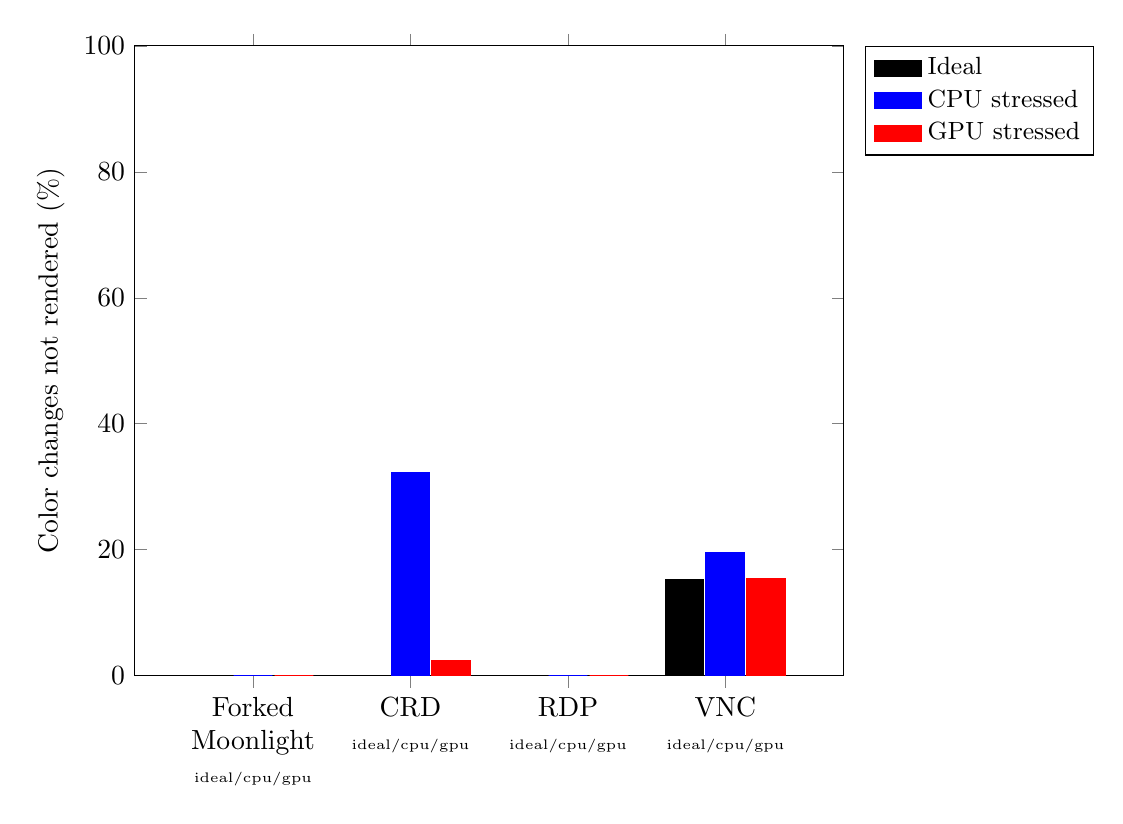
\begin{tikzpicture}
    \begin{axis}[
      ylabel={Color changes not rendered (\%)},
      scale only axis,
      height=8cm,
      width=\textwidth,
      enlarge x limits=0.25,
      ybar=2*\pgflinewidth,
      bar width=14pt,
      ymin=0,ymax=100,
      cycle list={{black},{blue},{red}},
      legend style={
          legend pos=outer north east,
          font=\small
        },
      legend cell align=left,
      legend image code/.code={%
          \draw[#1] (0cm,-0.1cm) rectangle (0.6cm,0.1cm);
        },
      % 1 unit in x controls the width:
      x=2cm,
      % ... and it means that we should describe intervals:
      xtick={0,1,2,...,10},
      % x tick label as interval,
      xticklabels={%
      {Forked Moonlight\\{\tiny ideal/cpu/gpu}},%
      {CRD\\{\tiny ideal/cpu/gpu}},%
      {RDP\\{\tiny ideal/cpu/gpu}},%
      {VNC\\{\tiny ideal/cpu/gpu}},%
      },
      x tick label style={
          text width=2.5cm,
          align=center
        },
      ]
      \addplot[style={black,fill=black,mark=none}]
      coordinates {(0, 0) (1,0) (2,0) (3,15.32)};

      \addplot[style={blue,fill=blue,mark=none}]
      coordinates {(0,0) (1,32.28) (2,0) (3,19.51)};

      \addplot[style={red,fill=red,mark=none}]
      coordinates {(0,0) (1,2.34) (2,0) (3,15.5)};

      \legend{Ideal,CPU stressed,GPU stressed}
    \end{axis}
  \end{tikzpicture}
  \caption[Color Delay Loss Data]{Percentage of color changes not rendered.}
  \label{fig:ColorDelayLoss}
\end{figure}

These data points adds context to the previous figures, showing where the applications struggle to keep up with sending data back to the client device.
The forked Moonlight implementation does not experience any frame drops, as does CRD under ideal conditions.
But once the host machine is put under heavy load, CRD begins to drop frames, with a few being dropped under GPU stress, and 32\% of frames being dropped while under CPU stress.
This can make CRD unpleasant and frustrating to use while the host is running a CPU intensive program as not only does the client take much more time to update the screen to reflect that status of the host computer, but many of the updates are lost completely and not shown to the user.
RDP is also able to display all the data sent by the host without dropping any frames under any condition.
VNC is again proved to be the least performant, with frames being dropped regardless of the load being put on the host computer.
This is still in line with it's intended use of basic remote control, though it is disappointing to see about 15\% loss even under ideal conditions.


\section{Quality}\label{sec:Quality}

Apart from the performance of each application, the quality of the user experience must also be taken into account when considering each application.
Each application will be assessed individually, and then compared in Section \ref{sec:EvaluationSummary}
When analyzing the forked version of Moonlight, specific quantitative data described in Section \ref{sec:DevelopingTestingAndMeasurementTools} can be collected directly from the application while it is running.
Once the streaming session concludes, the statistics are collated into human-readable numbers and presented in the console.
What follows is an example output from one of the test streaming sessions:

\begin{lstlisting}[style=plaintext,title=Statistics generated after a streaming session]
Global Video Stats
----------------------------------------------------------
Incoming frame rate from network: 62.18 FPS
Decoding frame rate: 62.18 FPS
Rendering frame rate: 62.18 FPS
Frames dropped by your network connection: 0.00%
Average network latency: 1 ms (variance: 0 ms)
Average decoding time: 4.27 ms
Average rendering time (including monitor V-sync latency): 0.06 ms


Total dropped frames: 0
\end{lstlisting}

This data shows that Moonlight is able to render all frames sent by the host without dropping any frames due to the network or decoding delays.
It is also able to keep the stream running at over 60 FPS throughout the entire session, which far exceeds the requirements of a pleasing to use system.
Taking into account the average frame decoding time of $4.27ms$ and the average rendering time of $0.06ms$, the program still has plenty of time in-between frames in case the streaming conditions are less favorable:
$(4.27ms+0.06ms) = 4.33ms < 16.\overline{66}ms = (\frac{1000ms}{60fps})$.
It is also worth noting that while testing the streaming quality, there were very few visual artifacts while monitoring the screen.
There were very few times where the screen appeared to be run through a compression filter, and it for the most part kept the visual fidelity of the host machine.

Chrome Remote Desktop also provides some quantitative data during streaming, which gives an insight into it's performance usage and speed. Figure \ref{fig:crdStats} shows screenshots of the stream during the most demanding test session.

\begin{figure}[h]
  % \centering
  % \begin{subfigure}{.25\textwidth}
  %   \centering
  %   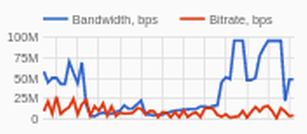
\includegraphics[width=1\linewidth]{Figures/crd/bandwidth}
  %   \caption{Bandwidth usage in bits per second}
  %   \label{fig:crdBandwidth}
  % \end{subfigure}%
  \begin{subfigure}{.33\textwidth}
    \centering
    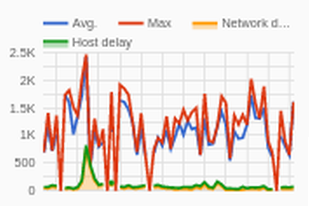
\includegraphics[width=1\linewidth]{Figures/crd/delay}
    \captionsetup{width=.85\linewidth}
    \caption{delay of image rendering in milliseconds}
    \label{fig:crdDelay}
  \end{subfigure}%
  \begin{subfigure}{.33\textwidth}
    \centering
    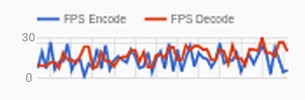
\includegraphics[width=1\linewidth]{Figures/crd/fps}
    \captionsetup{width=.85\linewidth}
    \caption{Frames per second encoded by host and decoded by client}
    \label{fig:crdFPS}
  \end{subfigure}%
  \begin{subfigure}{.33\textwidth}
    \centering
    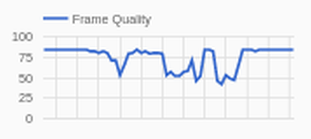
\includegraphics[width=1\linewidth]{Figures/crd/quality}
    \captionsetup{width=.85\linewidth}
    \caption{VP8 compression quality of current frames. Lower means CRD is struggling to keep up}
    \label{fig:crdQuality}
  \end{subfigure}
  \captionsetup{width=.8\linewidth}
  \caption[CRD Data]{Statistics from CRD during the most demanding test session. Data recorded over 60 seconds.}
  \label{fig:crdStats}
\end{figure}

Unfortunately, as there is no official documentation for this data, analysis on these figures is limited but insights on the stream quality can still be found.
As seen in Figure \ref{fig:crdDelay}, the delay of image rendering climbs as the CPU is put under stress, with frames sometimes taking entire seconds to be rendered on the client machine.
It is unclear on how much of the delay is due to the host machine versus the client machine, as the delay obviously rises as the host's CPU is put under stress, but it is clear that as the host machine is under heavy load the frames can take entire seconds to be rendered on the client machine.
Figure \ref{fig:crdQuality} shows the quality setting of the VP8 compression algorithm being adjusted over time to keep up with demand.
This is a decent indication of the quality of the video stream over time, as the quality drops in an attempt to keep the stream updating the client with as much frequency as possible instead of sending full frames.
With the knowledge that CRD leverages the VP8 compression algorithm \cite{miniorange_chromoting}, it is possible to infer that as the quality goes down, the frames being sent contain less information about the current frame and instead more temporal data to construct the new frame from the previous frame.
This is also seen with visual smudging on the client's screen as the stream slows down.

Microsoft's Remote Desktop Protocol does not provide quantitative data to analyze it's quality, but speaking from a user experience perspective, and considering the data provided in the previous section, RDP performed very well under each of the testing conditions.
By dropping zero frames and visually keeping up with the host machine, it is clear that RDP works extremely well over a local network.
Similar to Moonlight, there was very little loss of visual fidelity in the client's screen compared to the host's screen.
However, noticing that the bandwidth usage can climb upwards of 10 Mb/s, such streaming may cause issues while attempting to access the host machine while outside of the local network \cite{rdp_bandwidth}.
This will be further discussed in Section \ref{sec:ConclusionLimitations}.

VNC provides little in the form of quality statistics, but given it's performance and responsiveness discussed in the previous section, it is clear that the quality of the stream suffers heavily whenever the host is under load.
As discussed in Section \ref{subsec:VirtualNetworkComputing}, VNC was never built to be a highly performant protocol.
The testing done for this paper really stretches the limits of the protocol and pushes the use case of VNC to the extreme, but it is still worth looking into a common and widely used tool.

\section{Summary}\label{sec:EvaluationSummary}

By combining the information from the previous two sections, a wholistic picture of the performance of each application can be drawn. Firstly, Virtual Network Computing works as a bare-bones method of connecting to a host machine from a client device in the simplest way possible, but struggles at keeping up with even mildly demanding tasks.
As seen in Figure \ref{fig:ColorDelayLoss}, VNC failed to provide a smooth experience for the user even in ideal conditions by simply not rendering updates to the screen in time for the next frame to be shown.
This, combined with a slow response time and delayed inputs, causes a poor experience for the user when attempting to use demanding applications or anything that requires speed, making it unsuitable for the purposes of this paper.

Secondly, Chrome Remote Desktop performs well under ideal conditions and even succeeds at at maintaining steady performance under some GPU load, but it struggles to keep up whenever the host's CPU is under stress.
Due to CRD's reliance on web technologies, it too suffers from the same limitations as seen in other web streaming applications such as visual smearing and dependence on the CPU.
In fact, these issues are something technology companies like Google have been trying so solve, with the release of their new VP9 codec used for YouTube starting in 2014, but such technology has not yet been introduced to CRD \cite{google_io_vp9}.
Unfortunately, due to the dependence on the CPU, and difficulty in handling conditions where the host computer is running strenuous tasks, Chrome Remote Desktop is not a suitable software solution for the purposes of this paper.

Thirdly, Microsoft's Remote Desktop Protocol proves to be a very performant protocol that can handle nearly every situation without a problem.
It is slightly CPU limited, as seen in Figure \ref{fig:InputDelay}, but even then it is able to keep input latency under a very reasonable 40ms, and it still manages to render the host's screen without dropping any frames.
It even proves to be the most stable and consistent solution in Figure \ref{fig:ColorDelay}, producing the smallest variance in the render delay of the client's screen.
If it weren't for the limitations brought up in Section \ref{subsec:RemoteDesktopProtocol}, RDP would be a great solution for streaming demanding applications to a remote client.
However, because of these drawbacks, RDP is not suitable for every application.

Finally, Moonlight proves to be a high-performant solution that isn't limited by the host's CPU or GPU being under stress.
Each test resulted in highly similar results, and while it does on average have slightly higher response times compared to RDP (Figures \ref{fig:InputDelay} and \ref{fig:ColorDelay}), it only falls behind by 5-10ms -- quicker than the blink of an eye.
By not dropping any frames, and numerically proving it's ability to keep the stream above 60 frames per second, Moonlight proves to be a great solution for streaming demanding applications to a remote client without compromising its usability.